\documentclass[11pt,reqno]{amsart}

%%%%%%%%%%%%%%%%%%%%%%%%%%%%%%%%%%%%%%%%%%%%%%%%%%%
%								Packages									         %
%%%%%%%%%%%%%%%%%%%%%%%%%%%%%%%%%%%%%%%%%%%%%%%%%%%

\usepackage[T1]{fontenc}

\usepackage{amsmath}							
\usepackage{amssymb}
\usepackage{amsthm}
\usepackage{amscd}
\usepackage{amsfonts}
\usepackage{stmaryrd}
\usepackage{algorithm, algorithmic}
\usepackage{ wasysym }
\usepackage{caption}
\usepackage{subcaption}
\usepackage{euler}
\renewcommand{\rmdefault}{pplx}
\usepackage{extarrows}
\usepackage[colorlinks, linktocpage, citecolor = red, linkcolor = blue]{hyperref}
\usepackage{color}
\usepackage{tikz}									
\usepackage{fullpage}
\usepackage[shortlabels]{enumitem}
\usepackage{thmtools}


\linespread{1.1}

%%%%%%%%%%%%%%%%%%%%%%%%%%%%%%%%%%%%%%%%%%%%%%%%%%%
%								Theorems 								         %
%%%%%%%%%%%%%%%%%%%%%%%%%%%%%%%%%%%%%%%%%%%%%%%%%%%

\newtheorem{maintheorem}{Theorem}
\renewcommand*{\themaintheorem}{\Alph{maintheorem}}

\declaretheorem{FundamentalGroup}
\newtheorem{theorem}{Theorem}[section]
\newtheorem{lemma}[theorem]{Lemma}
\newtheorem{proposition}[theorem]{Proposition}
\newtheorem{corollary}[theorem]{Corollary} 
\newtheorem{conjecture}[theorem]{Conjecture} 

\theoremstyle{definition}
\newtheorem{maindefinition}[maintheorem]{Definition}								
\newtheorem{definition}[theorem]{Definition}
\newtheorem{question}[theorem]{Question}
\newtheorem{example}[theorem]{Example}
\newtheorem{construction}[theorem]{Construction}

%\theoremstyle{remark}
\newtheorem{remark}[theorem]{Remark}
\newtheorem{remarks}[theorem]{Remarks}
\newtheorem*{maintheorema}{Theorem \ref{thm:main}}


\renewcommand{\algorithmicrequire}{\textbf{Input:}}
\renewcommand{\algorithmicensure}{\textbf{Output:}}

%%%%%%%%%%%%%%%%%%%%%%%%%%%%%%%%%%%%%%%%%%%%%%%%%%%
%								Operators									         %
%%%%%%%%%%%%%%%%%%%%%%%%%%%%%%%%%%%%%%%%%%%%%%%%%%%


\newcommand{\madeline}[1]{{\color{purple} \sf  Madeline: [#1]}}

\newcommand{\R}{\mathbb{R}}
\newcommand{\C}{\mathbb{F}}
\newcommand{\F}{\mathbb{F}}
\newcommand{\nul}{\mathrm{null}}
\newcommand{\range}{\mathrm{range}}
\newcommand{\spa}{\mathrm{span}}



%%%%%%%%%%%%%%%%%%%%%%%%%%%%%%%%%%%%%%%%%%%%%%%%%%%
%                                                                          Title                                                                             %
%%%%%%%%%%%%%%%%%%%%%%%%%%%%%%%%%%%%%%%%%%%%%%%%%%%

\title{Quadratic Sieve}

\author[M. Carmona]{Marcos Carmona}
\address{Brown University,  Providence, RI 02912}
\email{\href{mailto:marcos_carmona@brown.edu}{marcos\_carmona@brown.edu}}



%%%%%%%%%%%%%%%%%%%%%%%%%%%%%%%%%%%%%%%%%%%%%%%%%%%%%%

\begin{document}


\maketitle
\setcounter{tocdepth}{1}
%\tableofcontents

%%%%%%%%%%%%%%%%%%%%%%%%%%%%%%%%%%%%%%%%%%%%%%%%%%%%%%
\section{Introduction}
The quadratic sieve factorization algorithm is an algorithm developed for integer factorization. Before the more complex number field sieve, it was considered the fastest factorization algorithm for large primes. The goal of the exploration is to understand how it works and the nuances/limitations of the algorithm. The structure of the paper will be as follows: we will first cover the algorithm itself, then we will go through an example, followed by a discussion on the limitations, failure rate, and runtime of the algorithm, and finally a brief discussion on my implementation of the algorithm in Python.


% %%%%%%%%%%%%%%%%%%%%%%%%%%%%%%%%%%%%%%%%%%%%%%%%%%%%%%
% \section{Background}
% \label{sec:background}

% In order to go through the algorithm, we must first understand a few of the ideas behind it. 

% \begin{definition}
%    A \textbf{quadratic residue} $r$ modulo a prime $p$ is an integer $r$ such that there exists another integer $x$ such that $x^2 \equiv r \pmod{p}$. In simpler terms, $r$ is a quadratic residue modulo $p$ if there exists an integer $x$ such that when $x$ is squared and divided by $p$, the remainder is $r$.
% \end{definition}

% \begin{definition}
%    Similarly, a \textbf{quadratic non-residue} $n$ modulo a prime $p$ is an integer $n$ such that there is no integer x satisfying $x^2 \equiv n \pmod{p}$. In other words, $n$ is a quadratic non-residue modulo $p$ if there is no integer $x$ such that when $x$ is squared and divided by $p$, the remainder is $n$.
% \end{definition}

%%%%%%%%%%%%%%%%%%%%%%%%%%%%%%%%%%%%%%%%%%%%%%%%%%%%%%
\section{Algorithm}
\label{sec:algorithm}
\setcounter{algorithm}{0}

The central idea behind the quadratic sieve is Fermat's idea of factorization via difference of squares. Let $N$ be some composite number. We know that if we can find some $a$ and $b$ such that $N + b^2 = a^2$, then $N = a^2 - b^2 = (a+b)(a-b)$. This gives us two factors of $N$, $a+b$ and $a-b$. 

\begin{lemma}
   If $x^2 - y^2 = kN$ and $N \nmid x\pm y$, then $\gcd(x - y, N)$ is a proper factor of N \cite{silverman2008introduction}.
\end{lemma}

\begin{proof}
   $(x-y)(x+y) = kN \rightarrow \frac{(x-y)(x+y)}{\gcd(x-y, N)} = \frac{kN}{\gcd(x-y, N)}$ which must be an integer because it divides both sides. $N \nmid x - y$, $\gcd(x-y, N) \neq N \rightarrow \gcd(x-y, N)$ is a proper factor of $N$ \cite{silverman2008introduction}.
\end{proof}

Thus, we only need to find $kN = a^2-b^2$ for some $k$. $kN \equiv 0 \pmod{N}$, which means we can simplify the problem to finding $a, b$ such that $a^2 \equiv b^2 \pmod{N}$, $a \neq b$. We can manually go through numbers until we find $a$, but this would take a long time. This is what the quadratic sieve algorithm aims to do but much much faster. The algorithm can be divided into 3 steps: relation building, elimination, and then GCD computation to get the final factor of $N$.

\subsection{Relation Building}

Our goal for this step is to find a large set of integers $a_1,...,a_r$ such that $c_i \equiv a_i^2 \pmod{N}$ is a product of small primes. The idea here is that $a_i^2$ and any product of $a_i^2$s, $A$, will be a perfect square, but critically $c_i \neq a_i^2$ in all cases because of the modulo (we actually pick the $a_i$ lower bound to be above $\sqrt{N}$ to guarantee this). So, if we can find a set of $c_i$ such that there product $C$ is a perfect square (them being products of small primes will help us do this), we have $C = B^2 \equiv A^2 \pmod{N}$, $A \neq B$, and $\gcd(N, A-B)$ is a proper factor of $N$.

\begin{definition}
   A positive integer $N$ is said to be \textbf{B-smooth} if all its prime factors are less than or equal to $B$. The number of $B$-smooth numbers less than T is given by $\psi(T, B)$ \cite{silverman2008introduction}.
\end{definition}

With this definition, we can formalize this idea of product of small primes by saying $c_i$ must be $B$-smooth for a boundary $B$. We can find these $a_i$ values with a sieving algorithm! Starting from $\lfloor \sqrt{N} \rfloor + 1$ up until some bound $X$, which is referred to in the literature as the sieving interval, we define a function $F(x) = x^2 - N$ and apply it to every number. For larger $N$, this multiple polynomials can be used to increase efficiency and effectiveness \cite{silverman1987multiple}.

\begin{definition}
   The \textbf{factor base} of $B$ is the set of primes less than $B$. In this paper, this set will also include all prime powers less than $B$ \cite{silverman2008introduction}.
\end{definition}

We want to calculate a large set of these $F(x)$ values; however, when factoring large numbers, the numbers between $\lfloor \sqrt{N} \rfloor + 1$ to $X$ will reach sizes that make it computationally infeasible to calculate the function for all possible $x$ values (without taking unreasonably long). Thus, we can strategically choose to calculate $F(x)$ only for $x$ values that we know will produce a product of one of the primes in the factor base. We know by congruence that if $x^2 \equiv N \pmod{p}$, where $p$ is a prime in the factor base, then $p$ divides $x^2 - N$. Additionally, if this equivalence has no solutions, we can disregard $p$ because we know it will not divide any number produced by $F(x)$.

Unless $p = 2$ (for which there is only one solution), for every prime, a number either not a quadratic residue (there exists an integer $x$ such that when $x$ is squared and divided by $p$, the remainder is $r$) or there are 2 solutions $\alpha_p, \beta_p$ such that $x^2 \equiv N \pmod{p}$. Thus, if we can find these solutions, we know that $p$ will divide every number $F(\alpha + ip)$ and $F(\beta + i)$, $i \in \mathbb{Z}, i > 0$. We can find these solutions via the Tonelli-Shanks algorithm. This algorithm is beyond the scope of this paper, but I utilize it in my implementation to find build the relations.

% This opens up a question of definitions of a factor base, since $3^3 = 27$ is a prime power larger than 11, but it is 11-smooth. The book defines the prime power version of a factor base as the set of primes and prime powers less than $B$, so the implication is that for the algorithm, while this will lead to some $B$-smooth numbers being disregarded, it is more efficient to only consider the primes and prime powers less than $B$ than have an infinite factor base (which would mean having to change the algorithm to account for this). The solution I can think of, and how I implemented it, is for every prime in the factor base, keep dividing the number in the list by the prime until it is no longer divisible.


\begin{definition}
   A \textbf{sieve} is method of producing a subset of elements that satisfy a certain property from a broader set by a certain process of elimination.
\end{definition} 

\begin{example}
   \textbf{Sieve of Eratosthenes}: Given a list of numbers from 2 to $n$, we can eliminate all multiples of 2, then all multiples of 3, then all multiples of 5, and so on. The remaining numbers are all prime. This generates all of the primes from 2 to $n$. 
\end{example}

So, iterating through all of the primes in the factor base, we use the Tonelli-Shanks algorithm to find all indices $x$ such that $F(x)$ has a factor in the list. Here's where the sieve comes in: for each number in this $F(x)$ list, we divide by every prime that it is divisible by (repeating in the case that it is divisible by a prime multiple times, representing prime powers). If the final result after we've gone through the factor base is 1 for a number, that number is B-smooth because all of its factors in the factor base. We then store every successful list of prime factors, the corresponding product, and the $x$ value that produced it. Using earlier terminology, $x_i$ is $a_i$ and $c_i$ is the product of the prime factors. 

\subsection{Elimination}
Now, our goal is to gather some combination of $a_i$s such that when we multiply all of their corresponding $c_i$s, they produce a perfect square (so all of their small factors are to an even power). We recall that we already gathered all of the factors when we determined that it was $B$-smooth, so this is equivalent to making a product of $c_i$s such that all of the small factors appear an even amount of times. In other words, for $c_{i_1}^{x_{i_1}} \cdots c_{i_s}^{x_{i_s}} \cdots c_{j_1}^{x_{j_1}} \cdots c_{j_k}^{x_{j_k}}$, where $c_{i_t}$ is the $t$th prime factor of a $c_i$, we want all $x_{i_\ell} \equiv 0 \pmod{2}$. This relation is not unique, and finding more of them increases the probability of finding a nontrivial factor, as we get more tries and potential factors \cite{silverman2008introduction}. 

We can solve this problem with linear algebra by setting up a system of equations and using linear algebra to find a solution. First, we write every $c_i$ in terms of all of the primes in the factor base, such that $c_i = p_1^{x_{i,1}} \ldots p_t^{x_{i, t}}$. 

Thus, we want to find $u_1,\ldots, u_r \in \{0, 1\}$ such that $c_1^{u_1}\cdots c_r{u_r} = p_1^{u_1 x_{1,1} + \cdots + u_r x_{r, 1}}\cdots p_t^{u_1 x_{1,t} \cdots u_r x_{r, t}}$ is a perfect square. We can write this as a matrix representing a system of equations under the field $\mathbb{F}_2$:

$$\begin{bmatrix}
   x_{1,1} & \ldots & x_{r, 1} \\
   \vdots & \ddots & \vdots \\
   x_{1, t} & \ldots & x_{r, t}
\end{bmatrix} \begin{bmatrix}
   u_1 \\
   \vdots \\
   u_r
\end{bmatrix} = \begin{bmatrix}
   0 \\
   \vdots \\
   0
\end{bmatrix}$$

We can solve this system of equations with Gaussian elimination. Note that $t$ is not necessarily equal to $r$. If $t = r$ then we have 1 solution, and if $t > r$, there will be multiple solutions. However, if $t > r$, we cannot find proper solutions, which is the $B$ bound must be sufficiently large. Once we have the $u$ vectors that serve as solutions, we can multiply the corresponding $c_i$s to get a perfect square. 

\subsection{GCD Computation}
Now, for each solution from the previous step, we have a set of $a_i$, whose product after squaring each is $A$, such that their corresponding $c_i \equiv a^2 \pmod{N}$, whose product $C$ is a perfect square $b^2$. Hopefully, $a - b \neq 0$. We compute the GCD of $A - C$ and $N$. We do this for all of the sets of $a_i$ we found in the elimination step and, hopefully, we find one of $N$'s nontrivial factors!

\subsection{Choosing B and X}
The two main bounds that determine how much we try is our $B$ bound and our $X$ bound, also referred to as the sieve interval and given as $[-M, M]$, with each bound being the lowest and highest $x$ fed into $F(x)$. The $B$ bound is arguably the most central to the algorithm, since for there to be solutions in the elimination step while factoring an integer $N$, $\psi(N, B) \geq \pi(B)$, the number of primes less than $B$. 

The proof-sketch behind the $B$ bound starts with the idea that checking if $a^2 \pmod{N}$ is $B$-smooth is equivalent to checking a random number. This approximation is actually overkill for the quadratic sieve, since by using the Tonelli-Shanks algorithm and looking only at $\alpha_p + ip$, the chances of hitting $B$-smooth numbers is increased.. You must check approximately $\frac{\pi(B)}{\psi(N, B)/N}$ random numbers to find $\pi(B)$ $B$-smooth numbers, which, by the prime number theorem and an additional corollary, is approximately $\frac{B/\ln{B}}{L(N)^{-\frac{1}{2}c}} = \frac{B}{\ln(B)L(N)^{-\frac{1}{2}c}}$, $L(N) = \exp(\sqrt{\ln N \ln \ln N})$ \cite{silverman2008introduction}.

To minimize how many numbers we check for smoothness, we want to select a $B$ that minizes that function. Since $L(N)$ is subexponential, we are content taking $B = L(N)^c$. Reducing, we get the equation $L(N)^{c+1/2c} \cdot \frac{1}{c\ln{L(N)}}$, which is minimized by $c = \frac{1}{\sqrt{2}}$. So we have $B = L(N)^{\frac{\sqrt{1}}{\sqrt{2}}}$ and the number of checks is $L(N)^{\sqrt{2}}$. With the Tonelli-Shanks approach to finding $B$-smooth numbers in the quadratic sieve, this is reduced to just $L(N)$ checks \cite{silverman2008introduction}.

The $X$ bound is less covered, but the number that I implemented as default came from a paper analyzing the runtime of the quadratic sieve algorithm that stated the optimal sieve interval is about $X = \exp(\sqrt{\ln N \ln \ln N})^{3\frac{\sqrt{2}}{4}}$ \cite{landquist2001quadratic}; however, the paper was also basing it off a slightly different $B$ bound of $B = \exp(\sqrt{\ln N \ln \ln N})^{\frac{\sqrt{2}}{4}}$, which likely impacted it. Like the $B$ bound, increasing sieve interval can increase the probability of finding a nontrivial factor, but it also increases the runtime of the algorithm, so it is a delicate balance.

%%%%%%%%%%%%%%%%%%%%%%%%%%%%%%%%%%%%%%%%%%%%%%%%%%%%%%
\section{Example}
\label{sec:example}

Let's go through an example of the quadratic sieve algorithm! We will factorize $N = 360379$. First, we need to choose our $B$ and $X$ bounds. For the sake of keeping numbers small, we can choose $B = 50$ and $X = 150$. We can find the factor base of 50 using the sieve of Eratosthenes or just checking numbers 1 to 50, which gives us the following factor base of 50: $\{2, 3, 5, 7, 11, 13, 17, 19, 23, 29, 31, 37, 41, 43, 47\}$. 

Now, we compute $\lfloor \sqrt{N} \rfloor + 1 = 601$, so we will consider numbers $x \in [601, 751]$. Now, using Tonelli-Shanks algorithm, we generate all of the possible valid $x$ and their corresponding $F(x)$ values, discarding primes with no solutions. We get the following list of $x$ and $F(x)$ values:
$[822, 2025, 3230, ..., 2973897, 2977550]$. 

%$[822, 2025, 3230, 4437, 5646, 6857, 8070, 9285, 10502, 11721, 12942, 14165, 15390, 16617, 17846, 19077, 20310,..., 2955662, 2959305, 2962950, 2966597, 2970246, 2973897, 2977550]$

Now, we go through the list of $F(x)$ values and divide by the primes in the factor base. Let's do an example with the first value: 822. 822 is divisible by 2, so we divide to $822 / 2 = 411$. Now, we get to 3. $411$ is divisible by 3, so we get $411 / 3 = 137$. However, if we go through the rest of the primes in the factor base, we notice that none of them divide it, so we'll have to discard 822. Now, let's try 3230. First, we divide by 2 to get 1615, then by 5 to get 323, then by 17 to get 19, and finally by 19 to get 1. Bingo! As an example for prime powers, 2025 is divisible by 3, so we divide by 3 to get 675, then by 3 again to get 225, and finally by 3 to get 75, which is divisible again by 3 to get 25, and finally by 5 to get 5, and 5 again to get 1. For both of these, we store the $x$ value that produced the $F(x)$ value, as well as the factors. We do this for all of these values, until we reach the end of the list. We now have a list of $a_i$, $a_i^2 = c_i$, and the small factors of $c_i$. 

$c_i$ factors: $[3, 3, 3, 3, 5, 5], [2, 5, 17, 19], [3, 3, 17, 29], ... [3, 5, 17, 17, 19, 29]$

%$[[3, 3, 3, 3, 5, 5], [2, 5, 17, 19], [3, 3, 17, 29], [2, 3, 3, 3, 3, 5, 19], [3, 3, 5, 19, 31], [2, 3, 5, 5, 5, 37], [5, 17, 29, 37], [3, 3, 19, 31, 37], [2, 3, 3, 5, 5, 17, 31], [2, 3, 3, 3, 17, 17, 17], [3, 5, 17, 31, 37], [3, 3, 3, 3, 17, 19, 19], [2, 3, 3, 5, 17, 19, 29], [2, 3, 3, 3, 5, 5, 29, 29], [3, 3, 5, 5, 5, 29, 37], [3, 17, 29, 29, 31], [3, 3, 5, 5, 19, 19, 29], [3, 5, 17, 17, 19, 29]]$

Now, we order the factor lists in increasing amount. We then make our exponent vectors modulo 2 (if a prime doesn't appear or appears an even amount of times in the factorization it is given a 0, otherwise it is given a 1), tracking how many times each prime is in the factorization of the $c_i$. 

Exponent vectors: $[0, 0, 0, 0, 0, 0, 0, 0], [1, 0, 1, 1, 1, 0, 0, 0], ..., [0, 0, 0, 0, 0, 1, 0, 0], [0, 1, 1, 0, 1, 1, 0, 0]$

%$[[0, 0, 0, 0, 0, 0, 0, 0], [1, 0, 1, 1, 1, 0, 0, 0], [0, 0, 0, 1, 0, 1, 0, 0], [1, 0, 1, 0, 1, 0, 0, 0], [0, 0, 1, 0, 1, 0, 1, 0], [1, 1, 1, 0, 0, 0, 0, 1], [0, 0, 1, 1, 0, 1, 0, 1], [0, 0, 0, 0, 1, 0, 1, 1], [1, 0, 0, 1, 0, 0, 1, 0], [1, 1, 0, 1, 0, 0, 0, 0], [0, 1, 1, 1, 0, 0, 1, 1], [0, 0, 0, 1, 0, 0, 0, 0], [1, 0, 1, 1, 1, 1, 0, 0], [1, 1, 0, 0, 0, 0, 0, 0], [0, 0, 1, 0, 0, 1, 0, 1], [0, 1, 0, 1, 0, 0, 1, 0], [0, 0, 0, 0, 0, 1, 0, 0], [0, 1, 1, 0, 1, 1, 0, 0]]$

With this, we set up the system of equations equating a product of some of the $c_i$ values to the 0 vector of the same length of primes in a factor base (because we need each exponent equal to 0 to get a perfect squares). We solve this Gaussian Elimination on the matrix \[
      \begin{bmatrix}
         0 & 0 & 0 & 0 & 0 & 0 & 0 & 0 \\
         1 & 0 & 1 & 1 & 1 & 0 & 0 & 0 \\
         \vdots \\
         0 & 0 & 0 & 0 & 0 & 1 & 0 & 0 \\
         0 & 1 & 1 & 0 & 1 & 1 & 0 & 0
      \end{bmatrix}
      \begin{bmatrix}
         u_1 \\
         u_2 \\
         \vdots \\
         u_7 \\
         u_8
      \end{bmatrix}
      =
      \begin{bmatrix}
         0 \\
         0 \\
         \vdots \\
         0 \\
         0
      \end{bmatrix}\]

The set of solutions to this is likely large, but we just have to keep trying different solutions until we find a nontrivial factor of $N$. For each candidate solution, let $A$ be the product of the $a_i$ values that correspond to solution variables that are 1, and similarly let $C$ be the product of the $c_i$ values that correspond to solution variables that are 1. We now have the congruence $A^2 \equiv C^2 \pmod{N}$, so we compute $\gcd(A - C, N)$. Suppose that we have already tried a few times until we get to the solution $u = [1, 1, 0, 0, 0, 0, 1, 1, 0, 0, 1, 0, 0, 1, 1, 1, 1, 0]$, which gives us $A = 482352584957531514725990400, C = 146894967184556442303172828822217149836914062500, A - C = -146894967184556442302690476237259618322188072100$. 

Computing $\gcd(360379, -14689496718455644230269047623725961832218807210)$, we get 557, which is a nontrivial factor of 360379, nice! This gives us our 2 factors, 557 and 647. 


%%%%%%%%%%%%%%%%%%%%%%%%%%%%%%%%%%%%%%%%%%%%%%%%%%%%%%
\section{Limitations, Failure Rate, and Runtime Analysis}
\label{sec:analysis}
% While no runtime is proven (CITE), there is a popular heuristic of the algorithm that is commonly accepted. The main deciding factor of determining the theoretical runtime of the quadratic sieve algorithm is the relation building step. The runtime of this step is $O(e^{\sqrt{\ln N \ln \ln N}})$ (%CITE https://www.fdi.ucm.es/profesor/m_alonso/Documentos/factorizacion/quadsieve.pdf).

% There may be proof (IF CITE FOUND)

% because of how we picked our $X$ bound (we have $X$ numbers to check) WRONG, as we saw in the last subsection, and the fact that in the quadratic sieve algorithm, we perform only a constant $\pi(B)$, which itself can be calculated with the sieve of Eratosthenes in less than $e^{\sqrt{\ln N \ln \ln N}}$ steps, divisions on each of those numbers in the worst possible case (where all the primes divide every number in the list), which is still a constant. This is the runtime of the entire sieving algorithm, since the elimination and GCD computation steps are both bounded under this step's runtime as essentially constant computational costs bounded under the sieve bound (by design of $B$, the number of solutions to calculate in the elimination step will always come accompanied by a larger computational cost in the sieve step, CITE/Elaborate here).

The accepted runtime heuristic for the quadratic sieve is directly based on the number of checks for $F(x)$ values, which we determined to be $\exp(\sqrt{\ln N \ln \ln N})$, since (when implemented optimally using techniques like block Wiedemann block algorithm), the other steps are bounded under the calculations. The two comparable algorithms, Pollard-Rho and the number field sieve, have different runtimes. Pollard-Rho has a runtime of $O(\sqrt{N})$ \cite{sutherland2007order}, and the number field sieve has a runtime of $\mathcal{O}(e^{c\sqrt[3]{(\ln N)(\ln \ln N)^{2}}})$ \cite{silverman2008introduction}, which has been determined to be approximately $\sqrt[3]{\frac{64}{9}}$ \cite{buhler1993factoring}.

The following graphic compares these $\mathcal{O}$ runtimes at just $N=5000000$:

\begin{center}
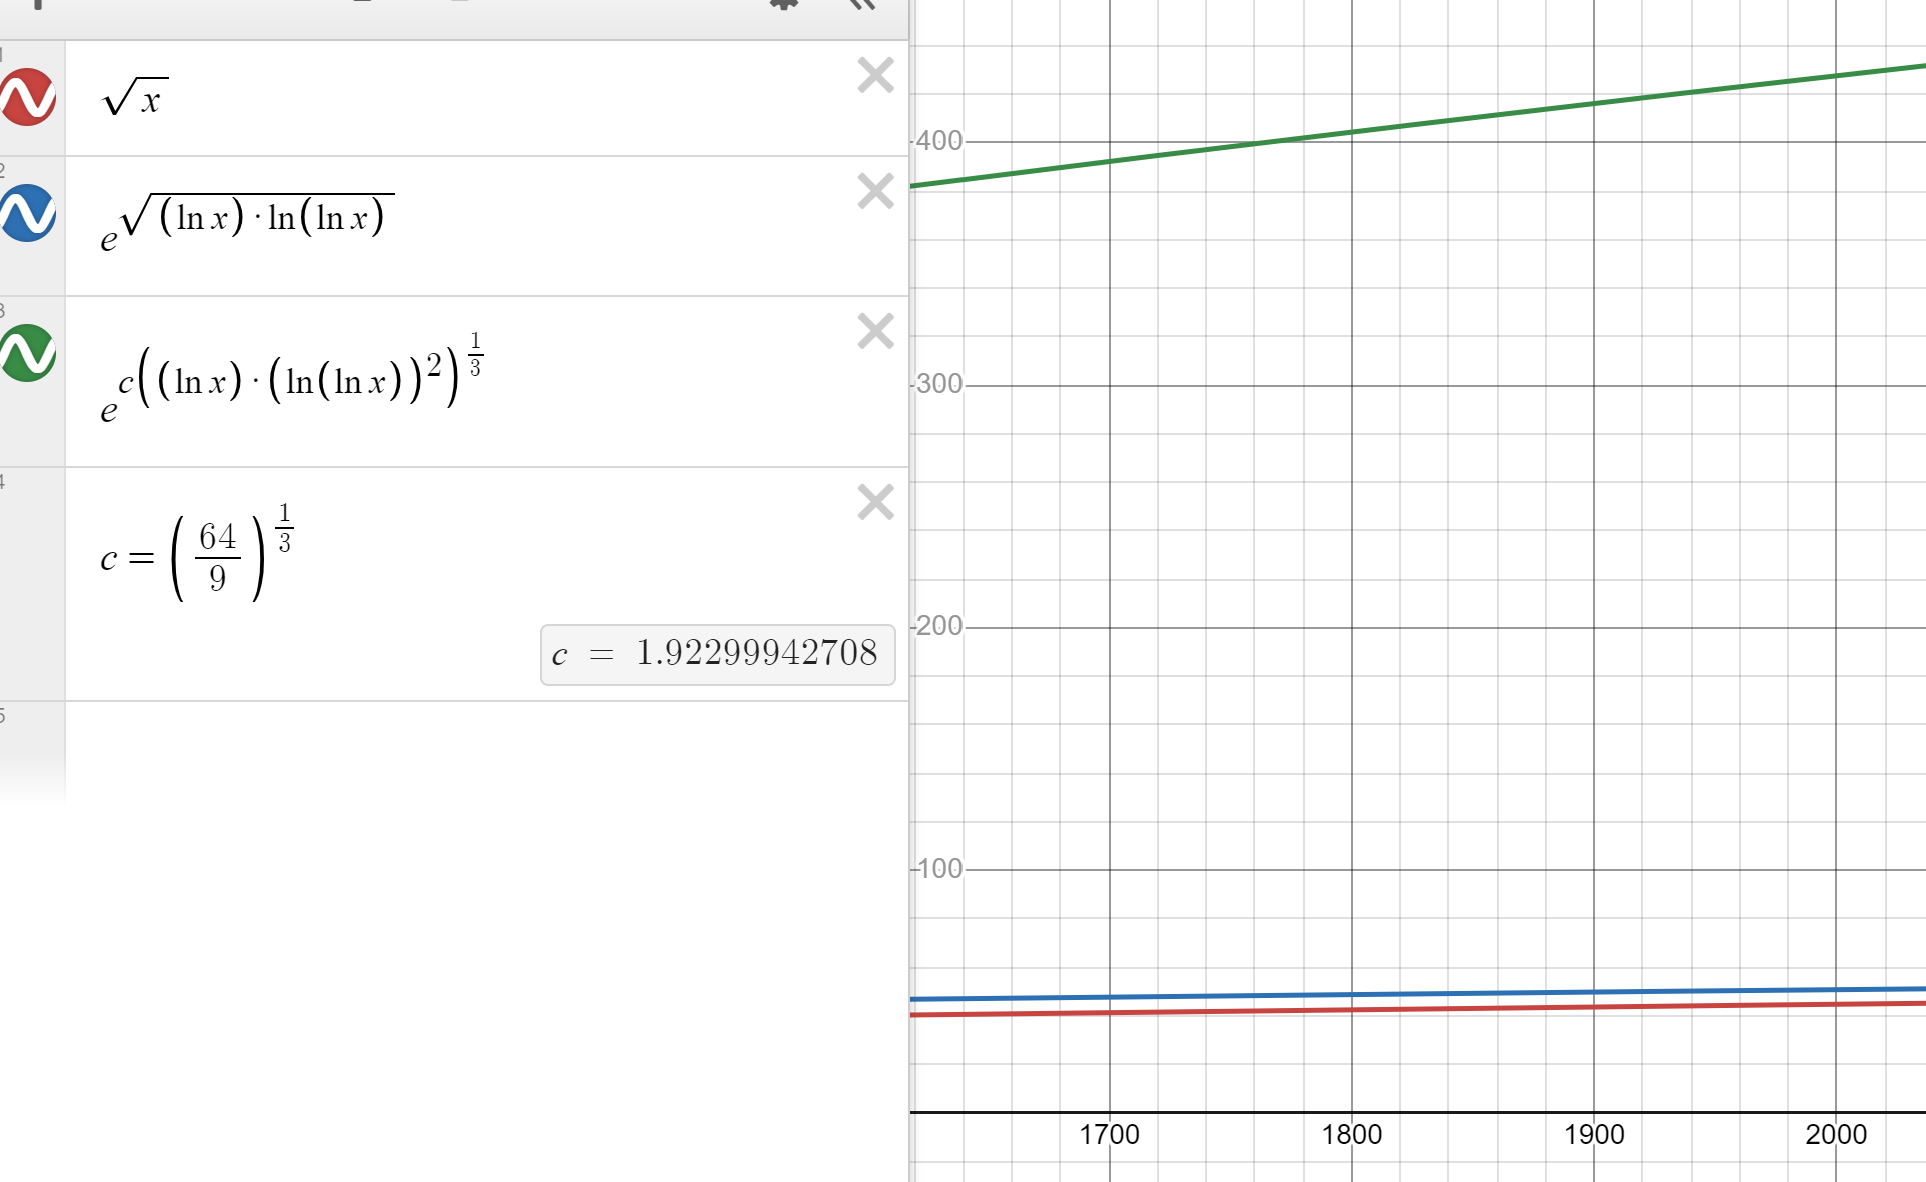
\includegraphics[scale=0.25]{runtimegraphic600.png}
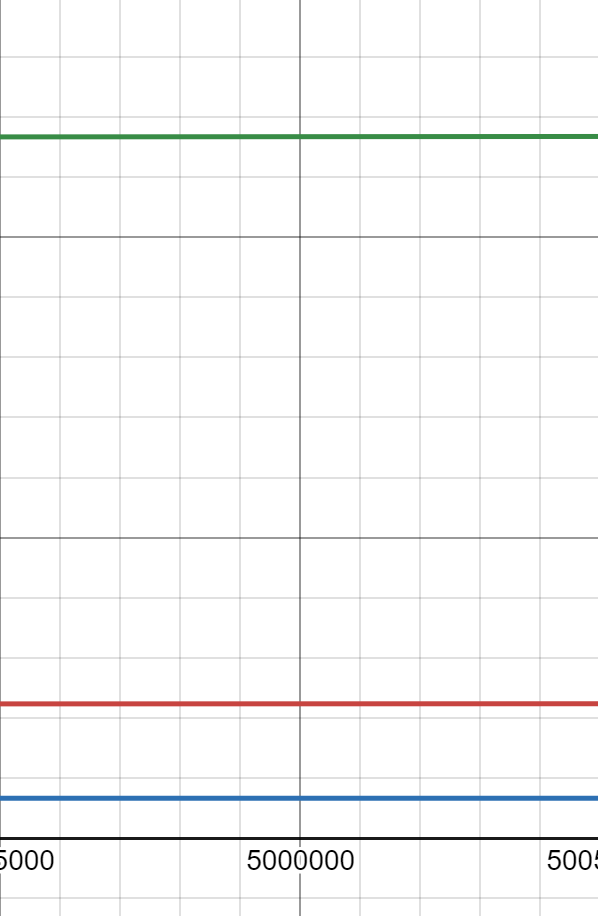
\includegraphics[scale=0.3]{runtimegraphic5000000.png}
\end{center}

As we can see, a superficial $\mathcal{O}$ misses costs that influence the runtime at different $N$ sizes. Because of constant factors, the actual case is that, broadly, pollard-rho is best for smaller $N$, around less than $10^{20}$, quadratic sieve is best for $N$ between $10^{20}$ and $10^{100}$, and the number field sieve is best for $N$ greater than $10^{100}$.

In truth, given the complexity and probabilistic nature of these algorithms, there is a lack of rigorous analysis of the runtime of these algorithms beyond heuristic estimates. Additionally, there is also a failure rate attributed to these algorithms that is difficult to calculate theoretically. Thus, we must rely on experimental results to give us a better idea of the runtime and failure rate of these algorithms.

Experimentally, we see that difference in bit size between factors is somewhat insignificant except for in extreme cases of a difference of 30-50 bits \cite{li2021empirical}. Additionally, we can measure "failure rate" by failure to factorize in an expected time (since otherwise, $B$ can be set arbitrarily high and factor anything in an unreasonable amount of time) despite optimal $B$ bounds, and we see that for large bit sizes, where both factors' bits add up to 60, it becomes only successful under 40\% of the time, decreasing even more with larger bit sizes \cite{li2021empirical}.

%%%%%%%%%%%%%%%%%%%%%%%%%%%%%%%%%%%%%%%%%%%%%%%%%%%%%%
\section{Implementation}

I'll keep this section brief since optimizing the python implementation was not the main focus of the project. My code is able to work for small composite numbers, and even that took over 250 lines of code. It turns out, coding quadratic sieve is difficult.

The issue that I couldn't fully fix was implementing Gaussian Elimination modulo 2 and extracting a basis of the vector space of all possible solutions. I ended up settling for the inefficient solution of generating all of the possible solutions and feeding them into my GCD computation step as they are generated using Python's yield instead of return. I included a failed implementation for a different algorithm using Gaussian Elimination that might be able generate a basis at the bottom of the code.

The other approach for elimination that I could've gone with is one that Silverman briefly mentions in the textbook. Since the matrices are very sparce, there are special algorithms that can handle them with higher efficiency, namely the block Wiedemann algorithm \cite{coppersmith1994solving}, but these were just outside of my coding ability.

Because of the flaws in the implementation, it is difficult to determine the runtime of my implementation, but I estimate it is magnitudes above the accepted heuristic. For one, in my implementation, I go through the primes and divide the list, meaning I need to traverse the list of $F(x)$ for every prime in the factor base, which is by construction is much greater than the number of primes in the factor base, so it would be more efficient to go the other way around and sieving while generating the list, stopping when the list is greater than $\pi(B)$. Additionally, the Gaussian Elimination step would usually be the shorter step, but given that I don't use a block algorithm and I produce redundant solutions, so in cases with high primes, this ends up taking a lot longer than the rest of the algorithm.

%%%%%%%%%%%%%%%%%%%%%%%%%%%%%%%%%%%%%%%%%%%%%%%%%%%%%%
\bibliographystyle{abbrv}
\bibliography{Bibliography}

\end{document}



